% tug-slides.tex: the .tex source for the slides for the presentation
% about Dednat6 at the TUG2018 meeting (slightly modified to need
% fewer dependencies).
%
% (find-angg "dednat6/tug-slides.tex")
% (defun c () (interactive) (find-dednat6sh "lualatex -record tug-slides.tex"))
% (defun d () (interactive) (find-pdf-page "~/dednat6/tug-slides.pdf"))
% (defun e () (interactive) (find-dednat6 "tug-slides.tex"))
% (defun l () (interactive) (find-dednat6 "myverbatim.lua"))
% (defun u () (interactive) (find-latex-upload-links "tug-slides"))
% (find-pdf-page   "~/dednat6/tug-slides.pdf")
% (find-sh0 "cp -v  ~/dednat6/tug-slides.pdf /tmp/")
% (find-sh0 "cp -v  ~/dednat6/tug-slides.pdf /tmp/pen/")
%   file:///home/edrx/dednat6/tug-slides.pdf
%                 file:///tmp/tug-slides.pdf
%             file:///tmp/pen/tug-slides.pdf
% http://angg.twu.net/dednat6/tug-slides.pdf

% «.defs»			(to "defs")
% «.verbatim»			(to "verbatim")
% «.myhbox»			(to "myhbox")
% «.bgcolorhbox»		(to "bgcolorhbox")
%
% «.title-page»			(to "title-page")
% «.dednat.icn»			(to "dednat.icn")
% «.dednat.icn-2»		(to "dednat.icn-2")
% «.dednat.icn-3»		(to "dednat.icn-3")
% «.dednat.icn-4»		(to "dednat.icn-4")
% «.dednat4.lua»		(to "dednat4.lua")
% «.dednat4.lua-diagram»	(to "dednat4.lua-diagram")
% «.dednat4.lua-diagram-2»	(to "dednat4.lua-diagram-2")
% «.dednat4.lua-diagram-3»	(to "dednat4.lua-diagram-3")
% «.dednat4.lua-diagram-4»	(to "dednat4.lua-diagram-4")
% «.dednat4.lua-diagram-5»	(to "dednat4.lua-diagram-5")
% «.dednat6»			(to "dednat6")
% «.dednat6-2»			(to "dednat6-2")
% «.dednat6-3»			(to "dednat6-3")
% «.download-test»		(to "download-test")
% «.extensions»			(to "extensions")
% «.hacking»			(to "hacking")
% «.eepitch-blocks»		(to "eepitch-blocks")
% «.repls»			(to "repls")
% «.repls-2»			(to "repls-2")
% «.hey»			(to "hey")

\documentclass[oneside]{book}
\usepackage[colorlinks,urlcolor=brown]{hyperref} % (find-es "tex" "hyperref")
\usepackage{amsmath}
\usepackage{amsfonts}
\usepackage{amssymb}
\usepackage{pict2e}
\usepackage{color}                % (find-dednat6 "edrx15.sty" "colors")
\usepackage{colorweb}             % (find-es "tex" "colorweb")
\usepackage{svgcolor}             % (find-es "tex" "svgcolor")
\usepackage{graphicx}
%
% (find-dn6 "preamble6.lua" "preamble0")
\usepackage{proof}   % For derivation trees ("%:" lines)
\input diagxy        % For 2D diagrams ("%D" lines)
%\xyoption{curve}     % For the ".curve=" feature in 2D diagrams
%
%
% (find-angg ".emacs.papers" "latexgeom")
% (find-dednat6file "2016-2-GA-VR.tex" "{geometry}")
% (find-latexgeomtext "total={6.5in,8.75in},")
\usepackage[paperwidth=11cm, paperheight=8.5cm,
            %total={6.5in,4in},
            %textwidth=4in,  paperwidth=4.5in,
            %textheight=5in, paperheight=4.5in,
            %a4paper,
            top=1.5cm, bottom=.5cm, left=1cm, right=1cm, includefoot
           ]{geometry}
%
\begin{document}

\catcode`\^^J=10
\directlua{dofile "dednat6load.lua"}  % (find-dednat6 "dednat6load.lua")




% «defs»  (to ".defs")
% I usually include these usepackages and inputs in my header:
%  \usepackage{edrx15}              % (find-LATEX "edrx15.sty")
%  \input edrxaccents.tex           % (find-LATEX "edrxaccents.tex")
%  \input edrxchars.tex             % (find-LATEX "edrxchars.tex")
%  \input edrxgac2.tex              % (find-LATEX "edrxgac2.tex")
%  \input edrxheadfoot.tex          % (find-LATEX "edrxheadfoot.tex")
% but I commented them out, and copied the relevant definitions
% here:

\def\noedrxfooter{}
\def\bsk{\bigskip}
\def\msk{\medskip}
\def\ssk{\smallskip}
\def\orange#1{{\color{orange}#1}}
\def\yellow#1{{\color{yellow}#1}}
\def\smashedvrule#1#2#3{\vrule width#1 height#2 depth#3 \kern-#1}
\def\bicolorhbox#1{{%
  \setbox0\hbox{#1}%
  \yellow{\smashedvrule{\wd0}{\ht0}{0pt}}%
  \orange{\smashedvrule{\wd0}{0pt}{\dp0}}%
  \box0%
  }}
\def\bhbox{\bicolorhbox}
\catcode`×=13 \def×{\times}
\catcode`Σ=13 \defΣ{\Sigma}
\catcode`λ=13 \defλ{\lambda}
\catcode`←=13 \def←{\ot}
\catcode`→=13 \def→{\to}
\catcode`♮=13 \def♮{\natural}
\def\id{\mathrm{id}}
\def\catA{\mathbf{A}}
\def\catB{\mathbf{B}}
\def\ot{\leftarrow}
\def\pbsymbol#1{%
  \begin{picture}(#1,#1)
    \put(0,0){\line(1,0){#1}}
    \put(#1,#1){\line(0,-1){#1}}
  \end{picture}}

% «verbatim» (to ".verbatim")
\directlua{dofile "myverbatim.lua"} % (find-dednat6 "myverbatim.lua")
\def\verbahbox#1{\hbox{\tt#1}}

% «myhbox» (to ".myhbox")
% (find-es "tex" "hbox")
\def\myhbox#1#2#3{\setbox0=\hbox{#3}\ht0=#1\dp0=#2\box0}
% \bhbox{\myhbox{7pt}{2pt}{\tt pb}}

\def\verbahbox#1{\myhbox{7pt}{2pt}{{\tt#1}}}

% «colors» (to ".colors")
% (find-dednat6 "2017ebl-slides.tex" "colors")
% (find-dednat6 "2017ebl-slides.tex" "colors" "\\def\\ColorGreen")
\long\def\ColorRed   #1{{\color{Red}#1}}
\long\def\ColorViolet#1{{\color{MagentaVioletLight}#1}}
\long\def\ColorGreen #1{{\color{SpringDarkHard}#1}}
\long\def\ColorGreen #1{{\color{SpringGreenDark}#1}}
\long\def\ColorGray  #1{{\color{GrayLight}#1}}

% (find-dednat6file "istanbulglyphs.el" "Bold:")
\catcode`𝐚=13 \def𝐚{\color{SpringGreenDark}}
\catcode`𝐛=13 \def𝐛{\color{black}}
\catcode`𝐠=13 \def𝐠{\color{SpringGreenDark}}
\catcode`𝐫=13 \def𝐫{\color{Red}}
\catcode`𝐧=13 \def𝐧{\color{blue}}
\catcode`𝐮=13 \def𝐮{\color{blue}}
\catcode`𝐜=13 \def𝐜{\color{pink}}
\catcode`𝐰=13 \def𝐰{\color{YellowOrangeLight}}

% «bgcolorhbox» (to ".bgcolorhbox")
% (find-dednat6 "edrx15.sty" "colors")
% (find-es "tex" "fbox")
\def\bgcolorhbox#1#2{{%
  \setbox0\hbox{#2}%
  \setbox0\vbox{\vskip\fboxsep\box0\vskip\fboxsep}%
  \setbox0\hbox{\kern\fboxsep\box0\kern\fboxsep}%
  {\color{#1}{\smashedvrule{\wd0}{\ht0}{\dp0}}}%
  \box0%
  }}

%\bgcolorhbox{blue}{Hello}
%\bgcolorhbox{YellowOrangeLight}{Hello}

\def\bgbox#1{\bgcolorhbox{YellowOrangeLight}{#1}}

\def\myvcenter#1{\begin{matrix}#1\end{matrix}}

\catcode`\^^O=13 \def{{\color{red}*}}









\setlength{\parindent}{0em}

%  _____ _ _   _                               
% |_   _(_) |_| | ___   _ __   __ _  __ _  ___ 
%   | | | | __| |/ _ \ | '_ \ / _` |/ _` |/ _ \
%   | | | | |_| |  __/ | |_) | (_| | (_| |  __/
%   |_| |_|\__|_|\___| | .__/ \__,_|\__, |\___|
%                      |_|          |___/      
%
% «title-page» (to ".title-page")
% (tugp 1)
% (find-es "tex" "huge")
% (find-kopkadaly4page (+ 12 63) "\\Huge")

\begin{tabular}[b]{c}
{\huge {\bf Dednat6: an extensible}} \\
{\LARGE {\bf (\ColorGreen{semi-})preprocessor for}} \\[1.5pt]
{\Large Lua\LaTeX{} that understands} \\
{\large diagrams \ColorGreen{in ASCII art}} \\
\\
%\includegraphics[width=2cm]{2018tug-edrx-hoop.png}\\
Eduardo Ochs - UFF \\
TUG 2018 - Rio de Janeiro, 20-22 jul 2018 \\
% \url{https://www.tug.org/tug2018/} \\
\url{http://angg.twu.net/dednat6.html} \\
% \url{http://angg.twu.net/math-b.html} \\
\end{tabular}

% https://www.tug.org/tug2018/ TUG2018



\newpage

\noedrxfooter


%      _          _             _         _            
%   __| | ___  __| |_ __   __ _| |_      (_) ___ _ __  
%  / _` |/ _ \/ _` | '_ \ / _` | __|     | |/ __| '_ \ 
% | (_| |  __/ (_| | | | | (_| | |_   _  | | (__| | | |
%  \__,_|\___|\__,_|_| |_|\__,_|\__| (_) |_|\___|_| |_|
%                                                      
% «dednat.icn» (to ".dednat.icn")
% (tugp 2)

{\bf Prehistory: dednat.icn}

My master's thesis was partly about Natural Deduction,

and it had lots of tree diagrams like these:

%L addabbrevs("->", "→")
%
%:  [x]^1  f     [a]^1  a->b
%:  --------     -----------
%:     f(x)   g       b       b->c
%:     --------       ------------
%:     g(f(x))             c
%:   ----------1         ----1
%:   λx.g(f(x))          a->c
%:
%:   ^x.g(f(x))          ^x.g(f(x)).t
%:
\pu
$$\ded{x.g(f(x))} \qquad \ded{x.g(f(x)).t}$$

I used \ColorGreen{\tt proof.sty} to typeset them, but the code

for each diagram was so opaque that I had to keep

a 2D ascii art version of each diagram in comments

so that I wouldn't get lost...


\newpage

% «dednat.icn-3» (to ".dednat.icn-3")
% (tugp 4)

{\bf Prehistory: dednat.icn (2)}

...like this:

\msk

%V %:  [x]^1  f     
%V %:  --------     
%V %:     f(x)   g  
%V %:     --------  
%V %:     g(f(x))   
%V %:   ----------1 
%V %:   λx.g(f(x))  
%V %:
%V $$\infer[{1}]{ \mathstrut λx.g(f(x)) }{
%V    \infer[{}]{ \mathstrut g(f(x)) }{
%V     \infer[{}]{ \mathstrut f(x) }{
%V      \mathstrut [x]^1 &
%V      \mathstrut f } &
%V     \mathstrut g } } }
%V $$

%L verbdef "foo"

\pu

$\quad
 \vcenter{\ded{x.g(f(x))}}
 \qquad
 \vcenter{\resizebox{!}{120pt}{\foo}}
$


\newpage

% «dednat.icn-2» (to ".dednat.icn-2")
% (tugp 4)

{\bf Prehistory: dednat.icn (3)}

...then I realized that I could automate the boring part.

I made the syntax of the 2D ascii art trees more rigid

and wrote a parser (in {\color{VioletDarkHard}Icon}!) that understood it.

A tree with a name tag like \ColorGreen{\tt \char`^foo} below it

would become a \ColorGreen{\tt \char`\\defded\{foo\}\{...\}} ---

\ColorRed{dednat.icn would only look for trees in `\ColorGreen{\tt \char`\%:}'-lines,}
%
%V %:  [x]^1  f    
%V %:  --------    
%V %:     f(x)   g 
%V %:     -------- 
%V %:     g(f(x))  
%V %:   ----------1
%V %:   λx.g(f(x)) 
%V %:
%V %:   ^foo
%
%L verbdef "footree"
%
%V \defded{foo}{
%V  \infer[{1}]{ \mathstrut λx.g(f(x)) }{
%V   \infer[{}]{ \mathstrut g(f(x)) }{
%V    \infer[{}]{ \mathstrut f(x) }{
%V     \mathstrut [x]^1 &
%V     \mathstrut f } &
%V    \mathstrut g } } }
%
%L verbdef "foodef"
%
\pu
$$
\myvcenter{\resizebox{!}{50pt}{\footree}}
\;\;\diagxyto/->/<200>\;\;
\myvcenter{\resizebox{!}{50pt}{\foodef}}
$$
%
and would put the `\ColorGreen{\tt \char`\\defded}'s in another file...


\newpage

% «dednat.icn-4» (to ".dednat.icn-4")
% (tugp 5)

{\bf Prehistory: dednat.icn (4)}

So that I could have this, in \ColorGreen{\tt myfile.tex}:
%
%V \input myfile.auto.dnt
%V %
%V %:  [x]^1  f    
%V %:  --------    
%V %:     f(x)   g 
%V %:     -------- 
%V %:     g(f(x))  
%V %:   ----------1
%V %:   λx.g(f(x)) 
%V %:
%V %:   ^foo
%V %
%V $$\ded{foo}$$
%
%L verbdef "footree"
%
\pu
$$
\myvcenter{\resizebox{!}{80pt}{\footree}}
\;\;\diagxyto/->/<200>\;\;
\myvcenter{\ded{x.g(f(x))}}
$$

Running `\ColorGreen{\tt dednat.icn myfile.tex}' would generate

the file \ColorGreen{\tt myfile.auto.dnt}.




\newpage

%  ____           _             _   _  _   
% |  _ \  ___  __| |_ __   __ _| |_| || |  
% | | | |/ _ \/ _` | '_ \ / _` | __| || |_ 
% | |_| |  __/ (_| | | | | (_| | |_|__   _|
% |____/ \___|\__,_|_| |_|\__,_|\__|  |_|  
%                                          
% «dednat4.lua» (to ".dednat4.lua")

{\bf Prehistory: dednat4.lua}

\ColorGreen{\tt dednat.icn} understood one kind of ``head'':

`\ColorGreen{\tt \%:}'-lines would be scanned for trees.

\msk

\ColorGreen{\tt dednat4.lua} understood three kinds of heads:

`\ColorGreen{\tt \%:}'-lines would be scanned for trees,

`\ColorGreen{\tt \%L}'-lines contained Lua code,

`\ColorGreen{\tt \%D}'-lines contained diagrams in a Forth-based language.

New heads could be added \ColorRed{dynamically}.

\bsk
\bsk
\bsk

{\scriptsize

(Actually I also had a head to define abbreviations
like `{\tt ->}' $→$ `{\tt \char`\\to\ }')

}

\newpage

% «dednat4.lua-diagram» (to ".dednat4.lua-diagram")


{\bf Dednat4.lua's language for diagrams}

Based on Forth: stack-based, and we can define words

that affect parsing --- that eat the next word or all

the rest of the line. Some words parse a 2D grid with

coordinates for nodes; other words join nodes with arrows.

Generates code for \ColorGreen{\tt diagxy.tex} (a front-end for \ColorGreen{\tt xypic}).

\def\BCCL{\mathsf{BCCL}}

%V %D diagram BCCL-std
%V %D 2Dx    100     +45                +55   +45
%V %D 2D 100 B0 <====================== B1
%V %D 2D     -\\                        -\\
%V %D 2D     | \\                       | \\
%V %D 2D     v  \\                      v  \\
%V %D 2D +20 B2 <\\> B2' ============== B3  \\
%V %D 2D      /\  \/                     /\  \/
%V %D 2D +15   \\   B4                    \\  B5
%V %D 2D        \\  -                      \\ -
%V %D 2D         \\ |                       \\|
%V %D 2D          \\v                        \v
%V %D 2D +20        B6 <===================== B7
%V %D 2D
%V %D 2D +10 b0 |---------------------> b1
%V %D 2D        |->                        |->
%V %D 2D +35        b2 |--------------------> b3
%V %D ((
%V %D    B0 .tex= f^{\prime*}P          B1 .tex= P
%V %D    B2 .tex= z^{\prime*}f^*Σ_zP    B3 .tex= z^*Σ_zP
%V %D    B4 .tex= Σ_{z'}f^{\prime*}P    B5 .tex= Σ_zP
%V %D    B6 .tex= f^*Σ_zP               B7 .tex= Σ_zP
%V %D     B2' .tex= f^{\prime*}z^*Σ_zP
%V %D    B0 B1 <-| B0 B2 -> B0 B2' -> B1 B3 -> B2 B2' <-> B2' B3 <-|
%V %D    B0 B4 |-> B1 B5 |->
%V %D    B2 B6 <-| B3 B7 <-|
%V %D    B6 B7 <-| B5 B7 -> .plabel= r \id
%V %D    B4 B6 -> sl_ .plabel= l ♮ B4 B6 <- sl^ .plabel= r \BCCL
%V %D    B0 B2' midpoint B1 B3 midpoint  harrownodes nil 20 nil <-|
%V %D    B0  B2 midpoint B4 B6 midpoint dharrownodes nil 20 nil |->
%V %D    B1  B3 midpoint B5 B7 midpoint dharrownodes nil 20 nil <-|
%V %D ))
%V %D (( b0 .tex= X×_{Y}Z b1 .tex= Z b2 .tex= X b3 .tex= Y
%V %D    b0 b1 -> .plabel= b f'
%V %D    b0 b2 -> .plabel= l z'
%V %D    b1 b3 -> .plabel= r z
%V %D    b2 b3 -> .plabel= a f
%V %D    b0 relplace 20 7 \pbsymbol{7}
%V %D ))
%V %D enddiagram
%V %
%V $$\diag{BCCL-std}$$
%
%L verbdef "BCCLstdsrc"



%D diagram BCCL-std
%D 2Dx    100     +45                +55   +45
%D 2D 100 B0 <====================== B1
%D 2D     -\\                        -\\
%D 2D     | \\                       | \\
%D 2D     v  \\                      v  \\
%D 2D +20 B2 <\\> B2' ============== B3  \\
%D 2D      /\  \/                     /\  \/
%D 2D +15   \\   B4                    \\  B5
%D 2D        \\  -                      \\ -
%D 2D         \\ |                       \\|
%D 2D          \\v                        \v
%D 2D +20        B6 <===================== B7
%D 2D
%D 2D +10 b0 |---------------------> b1
%D 2D        |->                        |->
%D 2D +35        b2 |--------------------> b3
%D 2D
%D ((
%D    B0 .tex= f^{\prime*}P          B1 .tex= P
%D    B2 .tex= z^{\prime*}f^*Σ_zP    B3 .tex= z^*Σ_zP
%D    B4 .tex= Σ_{z'}f^{\prime*}P    B5 .tex= Σ_zP
%D    B6 .tex= f^*Σ_zP               B7 .tex= Σ_zP
%D     B2' .tex= f^{\prime*}z^*Σ_zP
%D    B0 B1 <-| B0 B2 -> B0 B2' -> B1 B3 -> B2 B2' <-> B2' B3 <-|
%D    B0 B4 |-> B1 B5 |->
%D    B2 B6 <-| B3 B7 <-|
%D    B6 B7 <-| B5 B7 -> .plabel= r \id
%D    B4 B6 -> sl_ .plabel= l ♮ B4 B6 <- sl^ .plabel= r \BCCL
%D    B0 B2' midpoint B1 B3 midpoint  harrownodes nil 20 nil <-|
%D    B0  B2 midpoint B4 B6 midpoint dharrownodes nil 20 nil |->
%D    B1  B3 midpoint B5 B7 midpoint dharrownodes nil 20 nil <-|
%D ))
%D (( b0 .tex= X×_{Y}Z b1 .tex= Z b2 .tex= X b3 .tex= Y
%D    b0 b1 -> .plabel= b f'
%D    b0 b2 -> .plabel= l z'
%D    b1 b3 -> .plabel= r z
%D    b2 b3 -> .plabel= a f
%D    b0 relplace 20 7 \pbsymbol{7}
%D ))
%D enddiagram
%
\pu

\msk

$\quad
 \myvcenter{\resizebox{!}{80pt}{\BCCLstdsrc}}
 \;\;\diagxyto/->/<200>\;\;
 \myvcenter{\resizebox{!}{40pt}{$\diag{BCCL-std}$}}
$


\newpage

% «dednat4.lua-diagram-2» (to ".dednat4.lua-diagram-2")
% (tugp 8)

{\bf Dednat4.lua's language for diagrams (2)}

%V %D diagram adj
%V %D 2Dx     100    +25
%V %D 2D  100 LA <-| A
%V %D 2D      |      |
%V %D 2D      | <--> |
%V %D 2D      v      v
%V %D 2D  +25 B |-> RB
%V %D 2D
%V %D 2D  +15 \catB \catA
%V %D 2D
%V %D (( LA A <-|
%V %D    LA B -> A RB ->
%V %D    B RB |->
%V %D    LA RB harrownodes nil 20 nil <->
%V %D    \catB \catA <- sl^ .plabel= a L
%V %D    \catB \catA -> sl_ .plabel= b R
%V %D ))
%V %D enddiagram
%V %D
%V $$\diag{adj}$$
%
%L verbdef "adjsrc"

%D diagram adj
%D 2Dx     100   +25
%D 2D  100 LA    A
%D 2D
%D 2D  +25 B     RB
%D 2D
%D 2D  +15 \catB \catA
%D 2D
%D (( LA A <-|
%D    LA B -> A RB ->
%D    B RB |->
%D    LA RB harrownodes nil 20 nil <->
%D    \catB \catA <- sl^ .plabel= a L
%D    \catB \catA -> sl_ .plabel= b R
%D ))
%D enddiagram
%D

\msk

$\pu
  %\quad
  \myvcenter{\resizebox{!}{134pt}{\adjsrc}}
  \qquad
  \diag{adj}
$



\newpage

% «dednat4.lua-diagram-3» (to ".dednat4.lua-diagram-3")
% (tugp 9)

{\bf Dednat4.lua's language for diagrams (3)}

(See my ``Bootstrapping a Forth in 40 lines of Lua code''

in the Lua Gems book... section `Modes'')

% (find-angg ".emacs" "miniforth-article")

%V %D 𝐫diagram 𝐠adj
%V %D 𝐫2Dx𝐠     100    +25
%V %D 𝐫2D 𝐠 100 LA <-| A
%V %D 𝐫2D 𝐠     |      |
%V %D 𝐫2D 𝐠     | <--> |
%V %D 𝐫2D 𝐠     v      v
%V %D 𝐫2D 𝐠 +25 B |-> RB
%V %D 𝐫2D 𝐠
%V %D 𝐫2D 𝐠 +15 \catB \catA
%V %D 𝐫2D 𝐠
%V %D (( LA A <-|
%V %D    LA B -> A RB ->
%V %D    B RB |->
%V %D    LA RB 𝐫harrownodes 𝐠nil 20 nil 𝐛<->
%V %D    \catB \catA <- sl^ 𝐫.plabel= 𝐠a L
%V %D    \catB \catA -> sl_ 𝐫.plabel= 𝐠b R
%V %D ))
%V %D enddiagram
%V %D
%V $$\diag{adj}$$
%
%L verbdef "adjsrcb"

\msk

$\pu
  %\quad
  \myvcenter{\resizebox{!}{110pt}{\adjsrcb}}
  \;
  \begin{tabular}[c]{l}
  The words in {𝐫red} \\
  ``eat {𝐠text}''. \\
  {\tt𝐫2D} and {\tt𝐫2Dx} eat \\
  the rest of the line \\
  as a grid, and define \\
  nodes with coordinates. \\
  {\tt𝐫.plabel} modifies the \\
  arrow at the top of the \\
  stack: `{𝐠placement}' `{𝐠label}' \\
  \end{tabular}
  %\diag{adj}
$

\newpage

% «dednat4.lua-diagram-4» (to ".dednat4.lua-diagram-4")
% (tugp 10)

{\bf Dednat4.lua's language for diagrams (4)}

(See my ``Bootstrapping a Forth in 40 lines of Lua code''

in the Lua Gems book... section `Modes'')

% (find-angg ".emacs" "miniforth-article")

%V %D 𝐫diagram 𝐠adj
%V %D 𝐫2Dx𝐠     𝐜100    +25
%V %D 𝐫2D 𝐠 𝐜100 𝐧LA 𝐛<-| 𝐧A
%V %D 𝐫2D 𝐠     |      |
%V %D 𝐫2D 𝐠     | <--> |
%V %D 𝐫2D 𝐠     v      v
%V %D 𝐫2D 𝐠 𝐜+25 𝐧B 𝐛|-> 𝐧RB
%V %D 𝐫2D 𝐠
%V %D 𝐫2D 𝐠 𝐜+15 𝐧\catB \catA
%V %D 𝐫2D 𝐠
%V %D (( 𝐧LA A 𝐚<-|
%V %D    𝐧LA B 𝐚-> 𝐧A RB 𝐚->
%V %D    𝐧B RB 𝐚|->
%V %D    𝐧LA RB 𝐫harrownodes 𝐠nil 20 nil 𝐚<->
%V %D    𝐧\catB \catA 𝐚<- 𝐛sl^ 𝐫.plabel= 𝐠a L
%V %D    𝐧\catB \catA 𝐚-> 𝐛sl_ 𝐫.plabel= 𝐠b R
%V %D ))
%V %D enddiagram
%V %D
%V $$\diag{adj}$$
%
%L verbdef "adjsrcb"

\msk

$\pu
  \def𝐚{\color{green}}
  \def𝐚{\color{SpringGreenDark}}
  \def𝐛{\color{black}}
  \def𝐠{\color{black}} % {\color{SpringGreenDark}}
  \def𝐫{\color{black}} % {\color{Red}}
  \def𝐧{\color{blue}}
  \def𝐜{\color{MagentaDarkHard}}
  %\quad
  \myvcenter{\resizebox{!}{110pt}{\adjsrcb}}
  \;
  \begin{tabular}[c]{l}
  % The words in {𝐫red} \\
  % ``eat {𝐠text}''. \\
  {\tt𝐫2D} and {\tt𝐫2Dx} eat \\
  the rest of the line \\
  as a grid, and define \\
  {𝐧nodes} with {𝐜coordinates}. \\
  {𝐚Arrow words} connect the two \\
  topmost nodes in the stack. \\
  {\tt harrownodes} creates two \\
  phantom nodes for a middle \\
  horizontal arrow. \\
  \end{tabular}
  %\diag{adj}
$


\newpage

% «dednat4.lua-diagram-5» (to ".dednat4.lua-diagram-5")
% (tugp 11)

{\bf Dednat4.lua's language for diagrams (5)}

{\footnotesize

For the sake of completeness...
{𝐠\tt diagram} resets several tables,

{𝐠\tt enddiagram} outputs the table {\tt arrows} as diagxy code,

{𝐠\tt sl\char`^} and {𝐠\tt sl\char`_} slide the topmost arrow in the stack,

The `{𝐠\tt ))}' in a {𝐠\tt ((} $\ldots$ {𝐠\tt ))} block drops all top items from the

stack until the depth becomes what it was at the `{𝐠\tt ((}',

we can put Lua code in `{𝐠\tt \%L}' lines between `{𝐠\tt \%D}' lines, and...

}

%V require "diagforth"
%V 
%V storenode {TeX="a", tag="a", x=100, y=100}
%V storenode {TeX="b", tag="b", x=140, y=100}
%V = nodes
%V
%V storearrow(DxyArrow {from="a", to="b", shape="|->",
%V                      slide="5pt", label="up",
%V                      placement="a"})
%V storearrow(DxyArrow {from="a", to="b", shape=".>"})
%V storearrow(DxyPlace {nodes["a"]})
%V storearrow(DxyLiteral {"literal foobar"})
%V = arrows
%V
%V print(arrow_to_TeX(arrows[1]))
%V print(arrows[2]:TeX())
%V print(arrows[3]:TeX())
%V print(arrows[4]:TeX())
%V print(arrows_to_TeX())
%
%L verbdef "diaglua"

\msk

$\pu
  \myvcenter{\resizebox{!}{85pt}{\diaglua}}
  \;
  \begin{tabular}[c]{l}
  $𝐧←$ this Lua code \\
  shows how the \\
  low-level \\
  functions \\
  work... \\
  \\
  \end{tabular}
  %\diag{adj}
$

% (find-dn6 "diagforth.lua" "low-level-tests")




%%%%%%%%%%%%%%%%%%%%%%%%%%%%%%%%%%%%%%%%

\newpage

%  ____           _             _    __   
% |  _ \  ___  __| |_ __   __ _| |_ / /_  
% | | | |/ _ \/ _` | '_ \ / _` | __| '_ \ 
% | |_| |  __/ (_| | | | | (_| | |_| (_) |
% |____/ \___|\__,_|_| |_|\__,_|\__|\___/ 
%                                         
% «dednat6» (to ".dednat6")
% (tugp 12)

{\bf Dednat6: a semi-preprocessor}

Dednat4 is a real \ColorRed{pre-}processor ---

it generates a {\tt foo.auto.dnt} from {\tt foo.tex},

and it runs \ColorRed{before} \LaTeX.

\msk

In Dednat6 the Lua code that processes the

lines with heads like `{\tt𝐠\%L}', `{\tt𝐠\%:}', `{\tt𝐠\%D}', etc,

\ColorRed{pretends} to run \ColorRed{at the same time} as \TeX...

In fact there are synchronization points.

Each tree in a `{\tt𝐠\%:}' block generates a `{\tt𝐠\char`\\defded}'

each diagram in a `{\tt𝐠\%D}' block generates a `{\tt𝐠\char`\\defdiag}'...

`{\tt𝐠\char`\\pu}' means ``\ColorRed{process} all pending heads \ColorRed{until} the

current line'', and send the defs to \LaTeX ---


\newpage

% «dednat6-2» (to ".dednat6-2")
% (tugp 13)
% (find-dn6 "block.lua")

{\bf Dednat6: a semi-preprocessor (2)}

`{\tt𝐠\char`\\pu}' means ``\ColorRed{process} all pending heads \ColorRed{until} the

current line'', and send the defs to \LaTeX ---

This is implemented using ``blocks'' with {\tt i} and {\tt j} fields

for their starting and ending lines.


%V %D diagram triangle
%V %D 2Dx     100   +20
%V %D 2D  100 A --> B
%V %D 2D        \   |
%V %D 2D         v  v
%V %D 2D  +20       C
%V %D 2D
%V %D (( A B -> B C -> A C ->
%V %D ))
%V %D enddiagram
%V
%V $$\pu \diag{triangle}$$
%V
%V
%V %:  A  A->B  
%V %:  -------
%V %:     B      C
%V %:     --------
%V %:       B/\C
%V %:
%V %:       ^a-tree
%V %:
%V
%V $$\pu \ded{a-tree}$$
%
%L verbdef "diagramandtree"

\pu

\def\diagramandtreeexplan{
  \begin{tabular}[c]{l}
  {\tt tf = Block \{i=1, j=24, nline=1, ...\}} \\[5pt]
  First `{\tt𝐠\char`\\pu}': line 12 \\
  {\tt processuntil(12)} \\
  {\tt processlines(1, 11)} \\
  {\tt processblock \{head="{𝐠\%D}", i=1, j=10\}} \\
  {\tt output("\char`\\\char`\\defdiag\{{𝐠triangle}\}\{...\}")} \\
  {\tt nline=13} \\[5pt]
  {\tt tf} becomes {\tt\{i=1, j=24, nline=13, ...\}} \\[5pt]
  Second `{\tt𝐠\char`\\pu}': line 24 \\
  {\tt processuntil(24)} \\
  {\tt processlines(13, 23)} \\
  {\tt processblock \{head="{𝐠\%:}", i=15, j=22\}} \\
  {\tt output("\char`\\\char`\\defded\{{𝐠a-tree}\}\{...\}")} \\
  {\tt nline=25} \\
  \\
  \end{tabular}
}

$\myvcenter{\resizebox{!}{95pt}{\diagramandtree}}
  \quad
  \begin{tabular}[c]{l}
  `{\tt𝐠\%D}' block: lines 1--10 \\
  First `{\tt𝐠\char`\\pu}': line 12 \\
  `{\tt𝐠\%:}' block: lines 15--22 \\
  Second `{\tt𝐠\char`\\pu}': line 24 \\
  \\
  Whole .tex file: lines 1--24
  \end{tabular}
$


\newpage

% «dednat6-3» (to ".dednat6-3")
% (tugp 14)

{\bf Dednat6: a semi-preprocessor (3)}

% (find-dn6 "block.lua")
% (tuap 1)
% (tua)

`{\tt𝐠\char`\\pu}' means ``\ColorRed{process} all pending heads \ColorRed{until} the

current line'', and send the defs to \LaTeX ---

This is implemented using ``blocks'' with {\tt i} and {\tt j} fields

for their starting and ending lines.

\msk

\pu
$
  \myvcenter{\resizebox{!}{95pt}{\diagramandtree}}
  \;\;
  \resizebox{!}{50pt}{\diagramandtreeexplan}
$

\newpage

{\bf Dednat6: a semi-preprocessor (4)}

$
  \myvcenter{\resizebox{!}{140pt}{\diagramandtree}}
  \;\;
  \resizebox{!}{72pt}{\diagramandtreeexplan}
$




\newpage

%  ____                      _                 _      __  _            _   
% |  _ \  _____      ___ __ | | ___   __ _  __| |    / / | |_ ___  ___| |_ 
% | | | |/ _ \ \ /\ / / '_ \| |/ _ \ / _` |/ _` |   / /  | __/ _ \/ __| __|
% | |_| | (_) \ V  V /| | | | | (_) | (_| | (_| |  / /   | ||  __/\__ \ |_ 
% |____/ \___/ \_/\_/ |_| |_|_|\___/ \__,_|\__,_| /_/     \__\___||___/\__|
%                                                                          
% «download-test» (to ".download-test")
% (tugp 15)

{\bf Downloading and testing}

I gave up (temporarily?) keeping a package or a git repo

of Dednat6... but if you run something like this in a shell,

% (find-angg "dednat6/2017planar-has-1.tex")

%V rm -rfv /tmp/edrx-latex/
%V mkdir   /tmp/edrx-latex/
%V cd      /tmp/edrx-latex/
%V # See: http://angg.twu.net/LATEX/2017planar-has-1.pdf
%V wget   http://angg.twu.net/LATEX/2017planar-has-1.tgz
%V tar -xvzf 2017planar-has-1.tgz
%V lualatex  2017planar-has-1.tex
%
%L verbdef "downloadtest"

$\pu
  \myvcenter{\resizebox{!}{50pt}{\downloadtest}}
$

you download and unpack a .tgz with the full source code

for {\tt𝐠2017planar-has-1.pdf}, including a full version of

Dednat6, and all the (non-standard) \TeX{} files...

The home page of dednat6

\url{http://angg.twu.net/dednat6.html}

points to several such .tgzs, both simple and complex.


\newpage

%  _____      _                 _                 
% | ____|_  _| |_ ___ _ __  ___(_) ___  _ __  ___ 
% |  _| \ \/ / __/ _ \ '_ \/ __| |/ _ \| '_ \/ __|
% | |___ >  <| ||  __/ | | \__ \ | (_) | | | \__ \
% |_____/_/\_\\__\___|_| |_|___/_|\___/|_| |_|___/
%                                                 
% «extensions» (to ".extensions")
% (tugp 16)

{\bf Extensions}

It is easy to extend Dednat6 with new heads...

For example, for these slides I created a head `{\tt𝐠\%V}'

for a Dednat6-based verbatim mode...

the Lua code was initially just this:

%V registerhead "%V" {
%V   name   = "myverbatim",
%V   action = function ()
%V       local i,j,verbatimlinesorig = tf:getblock()
%V       verbatimlines = verbatimlinesorig
%V     end,
%V }
%
%L verbdef "verbatimhead"
$\pu
  \myvcenter{\resizebox{!}{50pt}{\verbatimhead}}
$

Dednat6 would take each block of `{\tt𝐠\%V}' lines and

store its contents in the global variable {\tt𝐠verbatimlines},

that I would process in Lua in `{\tt𝐠\%L}' lines to generate

the \LaTeX{} code that I want...

\newpage

%  _   _            _    _             
% | | | | __ _  ___| | _(_)_ __   __ _ 
% | |_| |/ _` |/ __| |/ / | '_ \ / _` |
% |  _  | (_| | (__|   <| | | | | (_| |
% |_| |_|\__,_|\___|_|\_\_|_| |_|\__, |
%                                |___/ 
% «hacking» (to ".hacking")

{\bf Hacking}

Hacking something usually consists of these stages:

1) ``reading'': understanding docs, data structures, code

2) making tests, dumping data structures

3) ``writing'': implementing new things

\msk

Here's how to do (1):

Learn a tiny bit of Emacs and eev:

\url{http://angg.twu.net/\#eev}

and run the ``eepitch blocks'' in the Lua source files...




\newpage

%  _____           _ _       _     
% | ____|___ _ __ (_) |_ ___| |__  
% |  _| / _ \ '_ \| | __/ __| '_ \ 
% | |__|  __/ |_) | | || (__| | | |
% |_____\___| .__/|_|\__\___|_| |_|
%           |_|                    
%
% «eepitch-blocks» (to ".eepitch-blocks")
% (find-dn6 "diagforth.lua" "low-level-tests")

{\bf Eepitch blocks in comments in Lua files}

This is a comment block in {\tt dednat6/diagforth.lua}:

%V --[==[
%V  (eepitch-lua51)
%V  (eepitch-kill)
%V  (eepitch-lua51)
%V require "diagforth"
%V storenode {TeX="a", tag="a", x=100, y=100}
%V storenode {TeX="b", tag="b", x=140, y=100}
%V = nodes
%V
%V storearrow(DxyArrow {from="a", to="b", shape="|->",
%V                      slide="5pt", label="up",
%V                      placement="a"})
%V storearrow(DxyArrow {from="a", to="b", shape=".>"})
%V storearrow(DxyPlace {nodes["a"]})
%V storearrow(DxyLiteral {"literal foobar"})
%V = arrows
%V
%V --]==]
%
%L verbdef "testa"
\pu
$\myvcenter{\resizebox{!}{80pt}{\testa}}
$

It is an ``e-script'' --- an {\sl executable log} of an experiment

that I was doing. It can be ``played back'' by typing

`F8's in Emacs+eev --- an `F8' on a red star line runs

that line as Lisp code ($→$ set up a target buffer)...

\newpage

{\bf Eepitch blocks in comments in Lua files (2)}

%V --[==[
%V  (eepitch-lua51)
%V  (eepitch-kill)
%V  (eepitch-lua51)
%V require "diagforth"
%V storenode {TeX="a", tag="a", x=100, y=100}
%V storenode {TeX="b", tag="b", x=140, y=100}
%V = nodes
%V
%V 𝐮(...)
%V --]==]
%
%L verbdef "testa"
\pu
$\myvcenter{\resizebox{!}{95pt}{\testa}}
$

An `F8' on a red star line runs that line as Lisp code

($→$ set up a target buffer with a Lua interpreter)

and an `F8' on a non-red star line sends that line to

the target buffer as if the user had typed it...


\newpage

%  ____  _____ ____  _         
% |  _ \| ____|  _ \| |    ___ 
% | |_) |  _| | |_) | |   / __|
% |  _ <| |___|  __/| |___\__ \
% |_| \_\_____|_|   |_____|___/
%                              
% «repls» (to ".repls")

{\bf REPLs}

Here's a screenshot.

\ssk

% (find-es "imagemagick" "convert")
% (find-sh0 "convert tug-slides-ss1.png -resize 200% tug-slides-ss2.png")
% (find-fline                "tug-slides-ss1.png")
% (find-fline                "tug-slides-ss2.png")
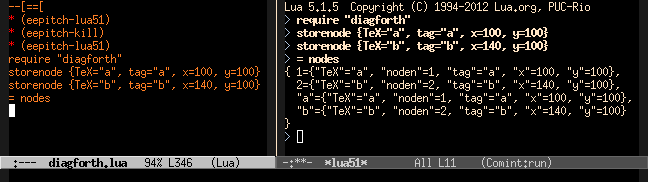
\includegraphics[width=240pt]{tug-slides-ss1.png}

{\footnotesize

Left Emacs window: the e-script buffer. The cursor is there:
{\color{RedOrangeDark}\vrule width 5pt height 7pt depth 1pt}.

We have just executed an eepitch block with `F8's.

\ssk

Right Emacs window: the target buffer, with a terminal

running Lua 5.1 in interactive (Read/Eval/Print/Loop) mode.

Blue `$𝐮>$'s: Lua prompts. Bold white: user input (sent with `F8's).

\ssk

{𝐫Here we used just Lua, not Lua\LaTeX.}

}

% (find-lua51manual "#6")

\newpage

%  _                                  _ 
% | |_   _  __ _       _ __ ___ _ __ | |
% | | | | |/ _` |_____| '__/ _ \ '_ \| |
% | | |_| | (_| |_____| | |  __/ |_) | |
% |_|\__,_|\__,_|     |_|  \___| .__/|_|
%                              |_|      
% «repls-2» (to ".repls-2")
% (find-dn6 "luarepl.lua")
% (find-dn6 "lua-repl/")
% (tugp 22)

{\bf REPLs (2)}

It is also possible to run Rob Hoelz's lua-repl

from inside Lua\LaTeX. Here's a screenshot.

% (find-fline                "tug-slides-sslr1.png")
%\includegraphics[width=220pt]{tug-slides-sslr1.png}
% (find-fline                "tug-slides-sslr1.png")
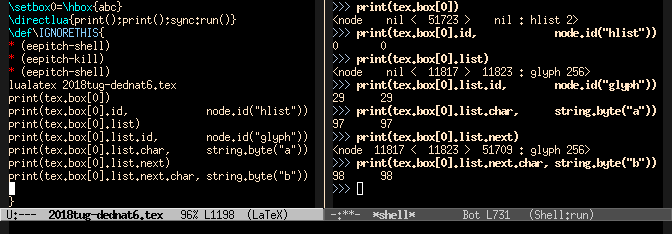
\includegraphics[width=240pt]{tug-slides-sslr2.png}

\setbox0=\hbox{abc}
%\directlua{print();print();sync:run()}
\def\IGNORETHIS{
 (eepitch-shell)
 (eepitch-kill)
 (eepitch-shell)
lualatex tug-slides.tex
print(tex.box[0])
print(tex.box[0].id,             node.id("hlist"))
print(tex.box[0].list)
print(tex.box[0].list.id,        node.id("glyph"))
print(tex.box[0].list.char,      string.byte("a"))
print(tex.box[0].list.next)
print(tex.box[0].list.next.char, string.byte("b"))

}

When you are a Bear of Very Little Brain ---

like me --- Lua\TeX's interface to \TeX{} boxes

looks very hard... lua-repl may help.


\newpage

%  _   _ _______   __
% | | | | ____\ \ / /
% | |_| |  _|  \ V / 
% |  _  | |___  | |  
% |_| |_|_____| |_|  
%                    
% «hey» (to ".hey")

{\bf \Large HEY!!!}

From \url{http://angg.twu.net/dednat6.html}:

\msk

I've stopped trying to document dednat6 because

1) I don't have a mental image of who I am writing for,

2) I get {\sl far too little feedback},

3) all of the feedback that I got came from people who felt that I was
not writing for them --- my approach, tone and choice of
pre-requisites were all wrong.

If you would like to try dednat6, get in touch, {𝐫let's chat} --- {\sl
  please}!

\msk

{\sl 
Maybe I can typeset in 20 minutes a diagram that took you

a day, maybe I can implement an extension that you need...
}





\end{document}



% Local Variables:
% coding: utf-8-unix
% End:
